% Main file. Venue is set entirely by the \usepackage[...] line below and
% the \trackname line further down -- swap those two spots to retarget a
% different evaluation-focused venue (TMLR, ICML/NeurIPS main track, a
% workshop). Section content lives in sections/*.tex and does not reference
% the venue at all, so it survives a venue swap unchanged.
%
% Default here: [eandd,preprint] -- readable, author name visible, NOT the
% anonymized submission format. Before an actual NeurIPS Evaluations &
% Datasets submission, switch to plain [eandd] (drops "preprint", restores
% double-blind anonymization) and run the anonymization pass this comment
% flags in sections/*.tex (self-references to "this project's own repo",
% the GitHub link, etc.).
\documentclass{article}
\usepackage[eandd,preprint]{neurips_2026}

\usepackage[utf8]{inputenc}
\usepackage[T1]{fontenc}
\usepackage{url}
\usepackage{booktabs}
\usepackage{graphicx}
\usepackage{amsmath}
\usepackage{amssymb}
\usepackage{nicefrac}
\usepackage{microtype}
\usepackage{xcolor}
\usepackage{multirow}

\graphicspath{{../../figures/}}

\usepackage{hyperref}
\hypersetup{colorlinks=true, linkcolor=blue, citecolor=blue, urlcolor=blue,
            pdftitle={What Can a Small Human Audit Establish About a Leaderboard Ranking?},
            pdfauthor={Rajveer Singh Pall}}

\newcommand{\code}[1]{\texttt{#1}}
\newcommand{\exactmatch}{\code{exact\_match}}
\newcommand{\scoreboxed}{\code{score\_boxed}}
% GENERATED by scripts/fb_rebuild_numbers.py -- do not edit by hand.
\newcommand{\nNRows}{22{,}508}
\newcommand{\nNDisagree}{817}
\newcommand{\nDisRate}{3.63\%}
\newcommand{\nDisLo}{3.39\%}
\newcommand{\nDisHi}{3.88\%}
\newcommand{\nDisMin}{0.60\%}
\newcommand{\nDisMax}{9.59\%}
\newcommand{\nSbOnly}{323}
\newcommand{\nEmOnly}{494}
\newcommand{\nNModels}{17}
\newcommand{\nNPairs}{136}
\newcommand{\nResPP}{3}
\newcommand{\nResJoint}{1}
\newcommand{\nResIndet}{0}
\newcommand{\nResSampling}{119}
\newcommand{\nWAuditJoint}{0.94}
\newcommand{\nWAuditPP}{0.72}
\newcommand{\nWSampling}{0.042}
\newcommand{\nRatioPP}{20.2}
\newcommand{\nRatioJoint}{25.5}
\newcommand{\nFalseCredits}{5}
\newcommand{\nNCredAud}{162}
\newcommand{\nFalseMiss}{0}
\newcommand{\nNWrongAud}{127}
\newcommand{\nAlphaHat}{0.0015}
\newcommand{\nAlphaLo}{0.0007}
\newcommand{\nAlphaHi}{0.0021}
\newcommand{\nAlphaFeas}{0.0023}
\newcommand{\nLR}{24.8}
\newcommand{\nLRp}{0.010}
\newcommand{\nLRlooStat}{6.1}
\newcommand{\nLRloop}{0.400}
\newcommand{\nIndetCred}{12}
\newcommand{\nIndetWrong}{19}
\newcommand{\nYiNineIndet}{8}
\newcommand{\nYiNineCred}{14}
\newcommand{\nNstarLow}{71}
\newcommand{\nNstarMid}{86}
\newcommand{\nNstarHigh}{160}
\newcommand{\nCurveFifty}{40\%}
\newcommand{\nCurveHundred}{55\%}
\newcommand{\nCurveTwoHundred}{73\%}
\newcommand{\nLabelsFifty}{1{,}700}
\newcommand{\nLabelsHundred}{3{,}400}
\newcommand{\nLabelsTwoHundred}{6{,}800}
\newcommand{\nSamplingCeiling}{87.5\%}
\newcommand{\nNBoot}{1000}
\newcommand{\nSingleComb}{0}
\newcommand{\nCeiling}{118}
\newcommand{\nCeilingSim}{103}
\newcommand{\nJointAudit}{101}
\newcommand{\nJointComb}{84}
\newcommand{\nJointSim}{76}
\newcommand{\nJointCombDrop}{84}
\newcommand{\nHetOne}{62}
\newcommand{\nHetTwo}{43}
\newcommand{\nHetThree}{26}
\newcommand{\nHetFive}{7}
\newcommand{\nHetTen}{0}
\newcommand{\nNoPool}{0}
\newcommand{\nPooledDisComb}{91}
\newcommand{\nCensusComb}{110}
\newcommand{\nCensusGapShrink}{9}
\newcommand{\nCensusGapShrinkCmdr}{5}
\newcommand{\nJointWidth}{0.086}
\newcommand{\nNPThreeK}{57}
\newcommand{\nNPLabelsFull}{27{,}200}
\newcommand{\nDesUniform}{88}
\newcommand{\nDesOneVer}{90}
\newcommand{\nDesConcOnly}{89}
\newcommand{\nDesBalanced}{95}
\newcommand{\nDesBalancedLo}{92}
\newcommand{\nDesBalancedHi}{98}
\newcommand{\nDesBalancedMin}{94}
\newcommand{\nDesBalancedMax}{95}
\newcommand{\nDesProp}{97}
\newcommand{\nDesFull}{97}
\newcommand{\nDesFullMin}{95}
\newcommand{\nDesFullMax}{97}
\newcommand{\nPowBalanced}{94\%}
\newcommand{\nPowBalancedMin}{77\%}
\newcommand{\nPowProp}{88\%}
\newcommand{\nPowPropMin}{65\%}
\newcommand{\nPowFull}{77\%}
\newcommand{\nPowFullMin}{47\%}
\newcommand{\nNRep}{200}
\newcommand{\nConcUpper}{1.9\%}
\newcommand{\nElevenUpper}{3.9\%}
\newcommand{\nZeroUpper}{2.5\%}
\newcommand{\nLOOCmdrP}{0.42}
\newcommand{\nLOOOtherPLo}{0.002}
\newcommand{\nLOOOtherPHi}{0.026}
\newcommand{\nCellElevenX}{141}
\newcommand{\nCellElevenN}{142}
\newcommand{\nCellTenX}{16}
\newcommand{\nCellTenN}{32}
\newcommand{\nCellTenDet}{20}
\newcommand{\nCellZeroOneX}{0}
\newcommand{\nCellZeroOneN}{1}
\newcommand{\nCellZeroX}{0}
\newcommand{\nCellZeroN}{145}
\newcommand{\nConcErr}{1}
\newcommand{\nConcN}{287}
\newcommand{\nScorerFlips}{8}
\newcommand{\nScorerFlipsSig}{7}
\newcommand{\nScorerFlipsCmdr}{6}
\newcommand{\nPointFlips}{2}
\newcommand{\nRShare}{94\%}
\newcommand{\nCurTotal}{289}
\newcommand{\nCurveEight}{50\%}
\newcommand{\nLabelsEight}{2{,}312}
\newcommand{\nCurveSixteen}{65\%}
\newcommand{\nLabelsSixteen}{4{,}624}
\newcommand{\nPlusLo}{7\%}
\newcommand{\nPlusHi}{15\%}
\newcommand{\nCmdrLR}{15.3}
\newcommand{\nLOOLo}{22.0}
\newcommand{\nLOOHi}{24.7}

\newcommand{\pending}[1]{\textcolor{red}{[PENDING --- human audit: #1]}}

\title{What Can a Small Human Audit Establish About\\
a Leaderboard Ranking? Two Verifiers and the\\
Assumption That Does the Work}

\author{
  Rajveer Singh Pall \\
  Department of Computer Science and Business Systems \\
  Gyan Ganga Institute of Technology and Sciences, Jabalpur, India \\
  \texttt{rajveerpall04@gmail.com}
}

\begin{document}

\maketitle

\begin{abstract}
Benchmark leaderboards report model accuracy as if it were an observed
quantity. It is the output of an automated verifier applied to free-text
generations, and that verifier can disagree with the correctness a human
reader would assign. We formalize this as a partial-identification problem:
given a benchmark's observed accuracy and an \emph{audited} estimate of the
verifier's false-credit and false-miss rates, we derive the sharp set of true
accuracy values consistent with the data, adapting classical
misclassification-bounds machinery \citep{manski1995identification} to
benchmark comparison. On MATH-Hard, using a real human audit of the standard
$\backslash$\texttt{boxed\{\}}-extraction comparator (400 items submitted, 350
usable across 27 models; a separate, later, targeted 69-item round on the
highest-priority models found zero additional scorer-wrong events, consistent
with---not contradicting---the pooled rate from the first round), we show that
\textbf{audit-estimation uncertainty---how little the verifier's own error
rate has been pinned down---exceeds sampling uncertainty for the majority of
model comparisons that remain identifiable at all} (median
identification-to-sampling width ratio $6.10\times$, 100\% dominant among 120
well-defined pairwise comparisons out of 136 candidates among 17 qualifying
models; a self-consistency check using the same audited comparator's own
accuracy rather than the field's reported metric gives $5.74\times$, also
100\% dominant---the two agree in direction and closely in magnitude, and the
minimum ratio across all 120 valid pairs is $2.15\times$, so the result is not
driven by a small number of extreme comparisons). We formalize the resulting
audit-budget allocation problem, prove the classical
\citep{neyman1934stratified} solution, and show empirically that its naive
plug-in form is \emph{dominated by uniform allocation} on this project's own
sparse real audit data---a documented failure mode with a tested correction. A
secondary finding: MATH-Hard's evaluation harness computes accuracy via two
live, independently-implemented extraction procedures that disagree on 3.63\%
of real responses (95\% CI [3.39\%, 3.88\%], $n=22{,}508$); we show this
scorer-choice dependence does not overturn the audit-estimation-dominance
finding, including under an adversarial worst-case bound, but establishes it
as a distinct, measurable source of benchmark uncertainty.
\pending{the verifier's other live scorer, \exactmatch\ via \code{math\_verify},
has not itself been human-audited; its own $\alpha,\beta$, and the fully
self-consistent identification result built on them, await a preregistered
458-row audit already in the field}.
\end{abstract}


\section{Introduction}
\label{sec:introduction}

A leaderboard number for a math benchmark is the output of a verifier: code
that extracts a final answer from free text and compares it with a
reference. Verifiers fail in known ways---unboxed answers, notation they
cannot normalize, text after the answer---and such failures led the Open LLM
Leaderboard to rescore its models with a new verifier
\citep{kydlicek2025fixing}. The usual safeguard is a human audit of a few
hundred responses, summarized as an error rate. Leaderboards exist to order
models, however, and an error rate that is small on average can still
reverse an ordering if it falls unevenly on one model.

We ask what a small audit can establish about orderings, using public
MATH-Hard generations from \nNModels{} models, the two verifiers the
evaluation harness runs on every response, and a 400-item human audit. We say
an ordering is \emph{resolved} when an interval for the difference in true
accuracy excludes zero at 95\% coverage under the stated assumptions.

\emph{Verifier choice reverses orderings} (Section~\ref{sec:results-census}).
Ranking by one verifier or the other reverses \nScorerFlips{} of \nNPairs{}
orderings; \nScorerFlipsSig{} are clear under both verifiers' sampling error.

\emph{Per-model auditing with one verifier resolves nothing}
(Section~\ref{sec:results-single}). The verifier is accurate on the audited
items, but each model contributes a handful of them, and the audit resolves
\nSingleComb{} orderings.

\emph{Verifier agreement concentrates the observed error}
(Section~\ref{sec:results-cells}). Where the two verifiers agree, the
transcribed human answer disagrees with them on \nConcErr{} of \nConcN{}
audited responses; the model-specific errors the audit finds are in the
disagreements.

\emph{What agreement buys depends on one assumption}
(Section~\ref{sec:results-joint}). If agreement is equally reliable across
models, the existing audit resolves \nJointComb{} of the \nCeiling{}
orderings sampling error permits. The count falls to \nHetTwo{} if each
model's agreement error may be twice the pooled bound, and to \nNoPool{}
without the assumption; the audit is too small to test it model by model.
The practical contribution is to make this assumption explicit, quantify how
much the ranking depends on it, and design the next audit to test it
(Section~\ref{sec:results-design}).

The estimators are classical \citep{neyman1938contribution,begg1983assessment};
the contributions are the measurements, the sensitivity analysis, and the
design they imply.

\section{Related Work}
\label{sec:related-work}

\paragraph{Two-phase sampling and verification bias.} Classifying everyone
cheaply and verifying a subsample stratified by the cheap result is
two-phase sampling \citep{neyman1938contribution}; \citet{tenenbein1970double}
treats misclassified binomial data including phase sizes, and
\citet{begg1983assessment} give the correction when verification depends only
on the test result. Our estimators are these. When the reference is instead
collected on units of known true status, sensitivity and specificity are the
natural parameters \citep{lang2014confidence}.

\paragraph{Hybrid human--automatic evaluation.} Prediction-powered inference
\citep{angelopoulos2023ppi} combines automatic labels with few human ones;
active \citep{zrnic2024active} and stratified \citep{fisch2024stratified}
variants choose what to label, the latter for language-model evaluation.
\citet{boyeau2025autoeval} apply the approach to model evaluation and
\citet{chatzi2024ranking} to rank sets of LLMs from pairwise preferences.
\citet{lee2026judge} correct one model's LLM-judge accuracy with sensitivity
and specificity estimated on calibration items drawn by true label, and
allocate those items between the two labels. Relative to these, we study
many models and all their pairwise orderings, allow error to differ by
model, and use agreement between two deterministic verifiers as the
stratifier.

\paragraph{Verifier reliability.} VerifyBench \citep{li2025verifybench} and
CompassVerifier \citep{liu2025compassverifier} compare verifiers' accuracy;
\citet{kydlicek2025fixing} document the extraction failures behind the Open
LLM Leaderboard \citep{fourrier2024openllm} rescoring;
\citet{biderman2024lessons} discuss evaluation reproducibility.

\paragraph{Concurrent work sharing data.} \citet{pall2026identified} (same
author, under review) uses the same audit and roster to bound accuracy by a
verifier's parse-failure count; its estimand and questions differ.

\section{Estimand and Identification}
\label{sec:setup}

\paragraph{Reference.} For model $m$ and item $i$, a human transcribes the
final answer the response commits to; $Y^\ast_{mi}=1$ if that transcription
is equivalent to the reference answer under the harness's normalization and
equivalence routine, and $Y^\ast_{mi}=0$ otherwise, including when the
response commits to no answer. The reference therefore validates
\emph{answer extraction}; equivalence errors shared by the verifiers and the
routine are not identified (Section~\ref{sec:data}). The target is
$A^\ast_m=P(Y^\ast=1)$ over the benchmark's items.

\paragraph{One verifier.} With verifier decision $\hat Y$ and accuracy
$a_m=P(\hat Y=1)$, known because the verifier runs on every item, an audit
stratified on $\hat Y$ estimates $q_m=P(Y^\ast=0\mid\hat Y=1)$ and
$r_m=P(Y^\ast=1\mid\hat Y=0)$, and
\begin{equation}
  A^\ast_m = a_m(1-q_m) + (1-a_m)\,r_m .
  \label{eq:identity}
\end{equation}
The error rates $\alpha_m=P(\hat Y=1\mid Y^\ast=0)=a_mq_m/(1-A^\ast_m)$ and
$\beta_m=P(\hat Y=0\mid Y^\ast=1)=(1-a_m)r_m/A^\ast_m$ follow by Bayes' rule;
feeding $q_m,r_m$ directly into the sensitivity/specificity correction
$(a-\alpha)/(1-\alpha-\beta)$ is biased and can return empty intervals
(Appendix~\ref{sec:appendix-sim}).

\paragraph{Two verifiers.} Each response falls in a joint cell
$c\in\{11,10,01,00\}$ (first index \code{score\_boxed}, second
\code{exact\_match}; 1 = credit). With census shares $s_{mc}$,
\begin{equation}
  A^\ast_m=\sum_c s_{mc}\,p_{mc},\qquad p_{mc}=P(Y^\ast=1\mid \text{cell } c,\ m).
  \label{eq:joint}
\end{equation}
$\Delta^\ast=A^\ast_1-A^\ast_2$ is linear in the $p_{mc}$, so over a box of
values its range is attained at corners and is sharp.

\paragraph{Assumptions compared.} Disagreement cells are always left
model-specific: $p_{m,10},p_{m,01}\in[0,1]$ unless audited. For the
concordant cells we compare
\begin{itemize}\itemsep1pt
  \item \emph{homogeneity}: $p_{m,11}=p_{11}$, $p_{m,00}=p_{00}$ for all
  models, estimated from the pooled audit;
  \item \emph{bounded heterogeneity} $L\ge1$: each model's
  $1-p_{m,11}$ and $p_{m,00}$ lie anywhere in $[0,\,L\cdot u]$, independently
  across models, where $u$ is the pooled upper confidence bound;
  \item \emph{no pooling}: each model's concordant rates from its own audited
  items only.
\end{itemize}
Pooling a single verifier's $(q,r)$ across models would instead give
$\Delta^\ast=(a_1-a_2)(1-q-r)$, whose sign never changes: it assumes away the
model-specific error that can reorder models.

\paragraph{Coverage.} For each ordering we split the 5\% error budget
between the audit (2.5\%) and benchmark sampling (2.5\%) and combine them by
the union bound, which needs no independence. Within the audit part, each
of the $k$ estimated parameters the ordering depends on gets a
Clopper--Pearson interval at level $0.975^{1/k}$; the estimates come from
disjoint samples, so they hold jointly with probability at least 0.975.
Parameters bounded logically ($[0,1]$) cost no coverage. The sampling part is
a normal interval for the difference in verifier accuracy. Details and a
simultaneous-over-all-orderings variant are in
Appendix~\ref{sec:appendix-coverage}.

\section{Data and Audit}
\label{sec:data}

\paragraph{Benchmark and verifiers.} MATH-Hard \citep{hendrycks2021math} on
the Open LLM Leaderboard v2 \citep{fourrier2024openllm}: 1{,}324 items in 7
subjects with public per-item generations. The harness scores every response
with \code{exact\_match}, which extracts the answer after a Minerva-style
``final answer'' phrase \citep{lewkowycz2022minerva} and is the leaderboard's
reported metric, and \code{score\_boxed}, which extracts the last
\verb|\boxed{}|. Both then apply the same normalization and equivalence
routine to the reference.

\paragraph{Human audit.} 400 (model, item) responses were drawn from 28
models' pooled responses, stratified by \code{score\_boxed} outcome
$\times$ subject $\times$ response-length quartile. Labelers saw the problem
and response only and transcribed the final answer the response commits to,
or marked it as committing to none (\code{NONE}) or to two unresolved answers
(\code{CONTRADICTORY}). The transcription is compared with the reference by
the verifiers' own equivalence routine, so the audit measures extraction
error; an equivalence error shared by the verifiers and the reference routine
is invisible to it. Three labelers overlapped on 151 and 75 items (Cohen's
$\kappa$ 0.61, 0.82, 0.79 across pairs).

\paragraph{Models and cells.} We use the \nNModels{} models with audited
items in both \code{score\_boxed} strata. Their audited responses fall in the
joint cells as in Table~\ref{tab:cells}. Because inclusion depends only on the
\code{score\_boxed} stratum, subject and length, it is independent of the
\code{exact\_match} outcome within a stratum, so the joint cells are valid
domains of the existing design.

\section{Results}
\label{sec:results}

\subsection{Verifier choice reverses orderings}
\label{sec:results-census}

The two verifiers disagree on \nNDisagree{} of \nNRows{} responses
(\nDisRate{}, 95\% CI [\nDisLo, \nDisHi]; \nEmOnly{} credited only by
\code{exact\_match}, \nSbOnly{} only by \code{score\_boxed}), from \nDisMin{}
to \nDisMax{} per model. Table~\ref{tab:reversals} lists the \nScorerFlips{}
orderings that reverse between them. \nScorerFlipsCmdr{} involve
\code{c4ai-command-r-v01}, which \code{exact\_match} scores at 0. The audit
contains few items per model, but in each case its evidence points the same
way: \code{command-r-v01}'s responses credited only by \code{score\_boxed}
are mostly wrong, as are \code{Yi-1.5-9B-Chat}'s (most commit to no answer),
while \code{zephyr-orpo} and \code{Qwen2-7B}'s are correct.

\begin{table}[t]
  \centering
  \caption{Orderings that reverse between the two verifiers. ``Sampling-clear'':
  the accuracy difference exceeds 1.96 standard errors under the named
  verifier(s). Last column: audited responses credited only by
  \code{score\_boxed} whose transcribed answer is correct, for each model.}
  \label{tab:reversals}
  \scriptsize
  \resizebox{\linewidth}{!}{\begin{tabular}{@{}lllcc@{}}
\toprule
Pair & higher by score\_boxed & higher by exact\_match & sampling-clear & audited sb-only correct/n \\
\midrule
Yi-1.5-9B-Chat vs zephyr-orpo-141b-A35b-v0.1 & Yi-1.5-9B-Chat & zephyr-orpo-141b-A35b-v0.1 & both & 1/9 ; 2/2 \\
Yi-1.5-9B-Chat vs Qwen2-7B & Yi-1.5-9B-Chat & Qwen2-7B & em only & 1/9 ; 2/2 \\
c4ai-command-r-v01 vs gpt-j-6b & c4ai-command-r-v01 & gpt-j-6b & both & 2/6 ; 0/0 \\
c4ai-command-r-v01 vs phi-2 & c4ai-command-r-v01 & phi-2 & both & 2/6 ; 0/0 \\
c4ai-command-r-v01 vs Mistral-7B-v0.1 & c4ai-command-r-v01 & Mistral-7B-v0.1 & both & 2/6 ; 0/0 \\
c4ai-command-r-v01 vs mpt-7b & c4ai-command-r-v01 & mpt-7b & both & 2/6 ; 0/0 \\
c4ai-command-r-v01 vs falcon-40b & c4ai-command-r-v01 & falcon-40b & both & 2/6 ; 0/0 \\
c4ai-command-r-v01 vs falcon-7b & c4ai-command-r-v01 & falcon-7b & both & 2/6 ; 0/1 \\
\bottomrule
\end{tabular}
}
\end{table}

\subsection{Per-model correction with one verifier resolves nothing}
\label{sec:results-single}

With \code{score\_boxed} and each model's own audited items, the audit finds
\nFalseCredits{} false credits in \nNCredAud{} credited items and \nFalseMiss{}
false rejections in \nNWrongAud{} rejected ones, and corrected point
estimates reorder only \nPointFlips{} pairs. Yet at 95\% coverage the audit
resolves \nSingleComb{} orderings, against \nCeiling{} that sampling error
alone permits (Appendix~\ref{sec:appendix-single}, Figure~\ref{fig:intervals}).
\nRShare{} of each model's interval width comes from the rejected stratum:
zero observed errors in 1--17 items bounds $r_m$ only loosely, and the
rejected stratum holds most of each model's responses. Simulated
single-verifier audits resolve half the orderings at about \nLabelsEight{}
labels (Appendix~\ref{sec:appendix-single}). Plug-in Neyman allocation
resolves none at any budget, because zero-event pilot strata receive no
labels.

\subsection{Where verifier error concentrates}
\label{sec:results-cells}

\begin{table}[t]
  \centering
  \caption{Audited responses of the \nNModels{} models by joint verifier cell,
  and how many have a transcribed answer equal to the reference (responses
  committing to no answer count as not equal).}
  \label{tab:cells}
  \small
  \begin{tabular}{@{}lcccc@{}}
    \toprule
    Cell & both credit & both reject & \code{score\_boxed} only & \code{exact\_match} only \\
    \midrule
    Audited & \nCellElevenN & \nCellZeroN & \nCellTenN & \nCellZeroOneN \\
    Transcription correct & \nCellElevenX & \nCellZeroX & \nCellTenX & \nCellZeroOneX \\
    \bottomrule
  \end{tabular}
\end{table}

Where the verifiers agree, the transcribed answer disagrees with them on
\nConcErr{} of \nConcN{} audited responses; the exact 95\% upper bound on
this rate is \nConcUpper{} (\nElevenUpper{} and \nZeroUpper{} for the two
concordant cells separately). This is a low observed rate with a finite-sample
bound, not proof that agreement is reliable, and it says nothing about
whether the rate is the same for every model. Where \code{score\_boxed}
credits and \code{exact\_match} does not, \nCellTenX{} of \nCellTenN{}
transcriptions are correct (Table~\ref{tab:cells}); every false credit of
\code{command-r-v01} is in this cell. The \code{exact\_match}-only cell has
493 responses in the population but \nCellZeroOneN{} audited, because the
audit was stratified on \code{score\_boxed}.

\subsection{What verifier agreement buys, and what it assumes}
\label{sec:results-joint}

\begin{figure}[t]
  \centering
  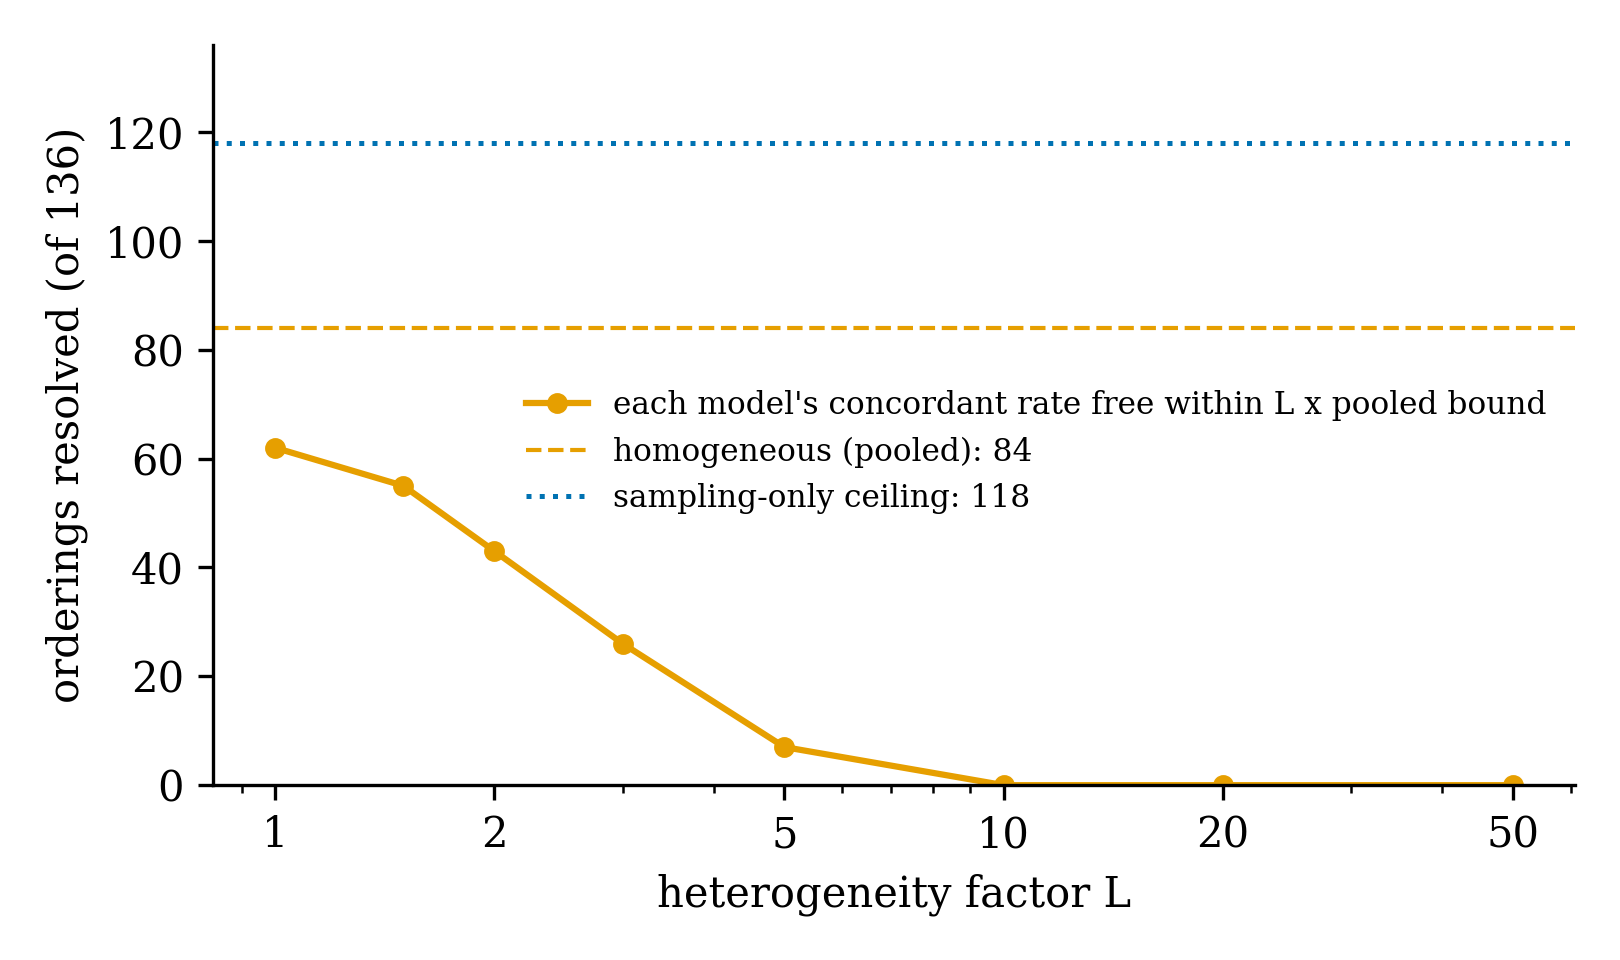
\includegraphics[width=0.66\linewidth]{figE_homogeneity_sensitivity.png}
  \caption{Orderings resolved by the existing audit, at 95\% coverage per
  ordering, as the concordant-cell assumption is relaxed. Dashed: concordant
  error homogeneous across models. Solid: each model's concordant error free
  within $L$ times the pooled bound. Dotted: orderings that sampling error
  alone permits.}
  \label{fig:assumption}
\end{figure}

Under homogeneity, with disagreement cells left model-specific and bounded
only by $[0,1]$, the existing audit resolves \nJointComb{} of the \nCeiling{}
orderings sampling permits (\nJointAudit{} of \nNPairs{} from the audit
alone; \nJointSim{} of \nCeilingSim{} with coverage simultaneous over all
orderings; \nJointCombDrop{} if responses without a committed answer are
dropped rather than counted as incorrect). Figure~\ref{fig:assumption} shows
how much of this is the assumption. If each model's concordant error may lie
anywhere within the pooled bound ($L=1$), \nHetOne{} orderings remain; at
$L=2$, \nHetTwo; at $L=5$, \nHetFive; at $L=10$, \nHetTen. With no pooling at
all the count is \nNoPool{}. Recovering \nJointComb{} without the assumption
would require about \nNPLabelsFull{} concordant labels (\nNPThreeK{} at
3{,}400), because every model's two concordant cells, which hold most of its
responses, would need their own tight bounds.

The assumption is plausible on mechanism: two extractors that read answers
in different ways and return the same verdict rarely both err on the same
response. The audit cannot confirm it model by model: models have 0 to 37
audited items per concordant cell.

\subsection{Designing the next audit}
\label{sec:results-design}

\begin{figure}[t]
  \centering
  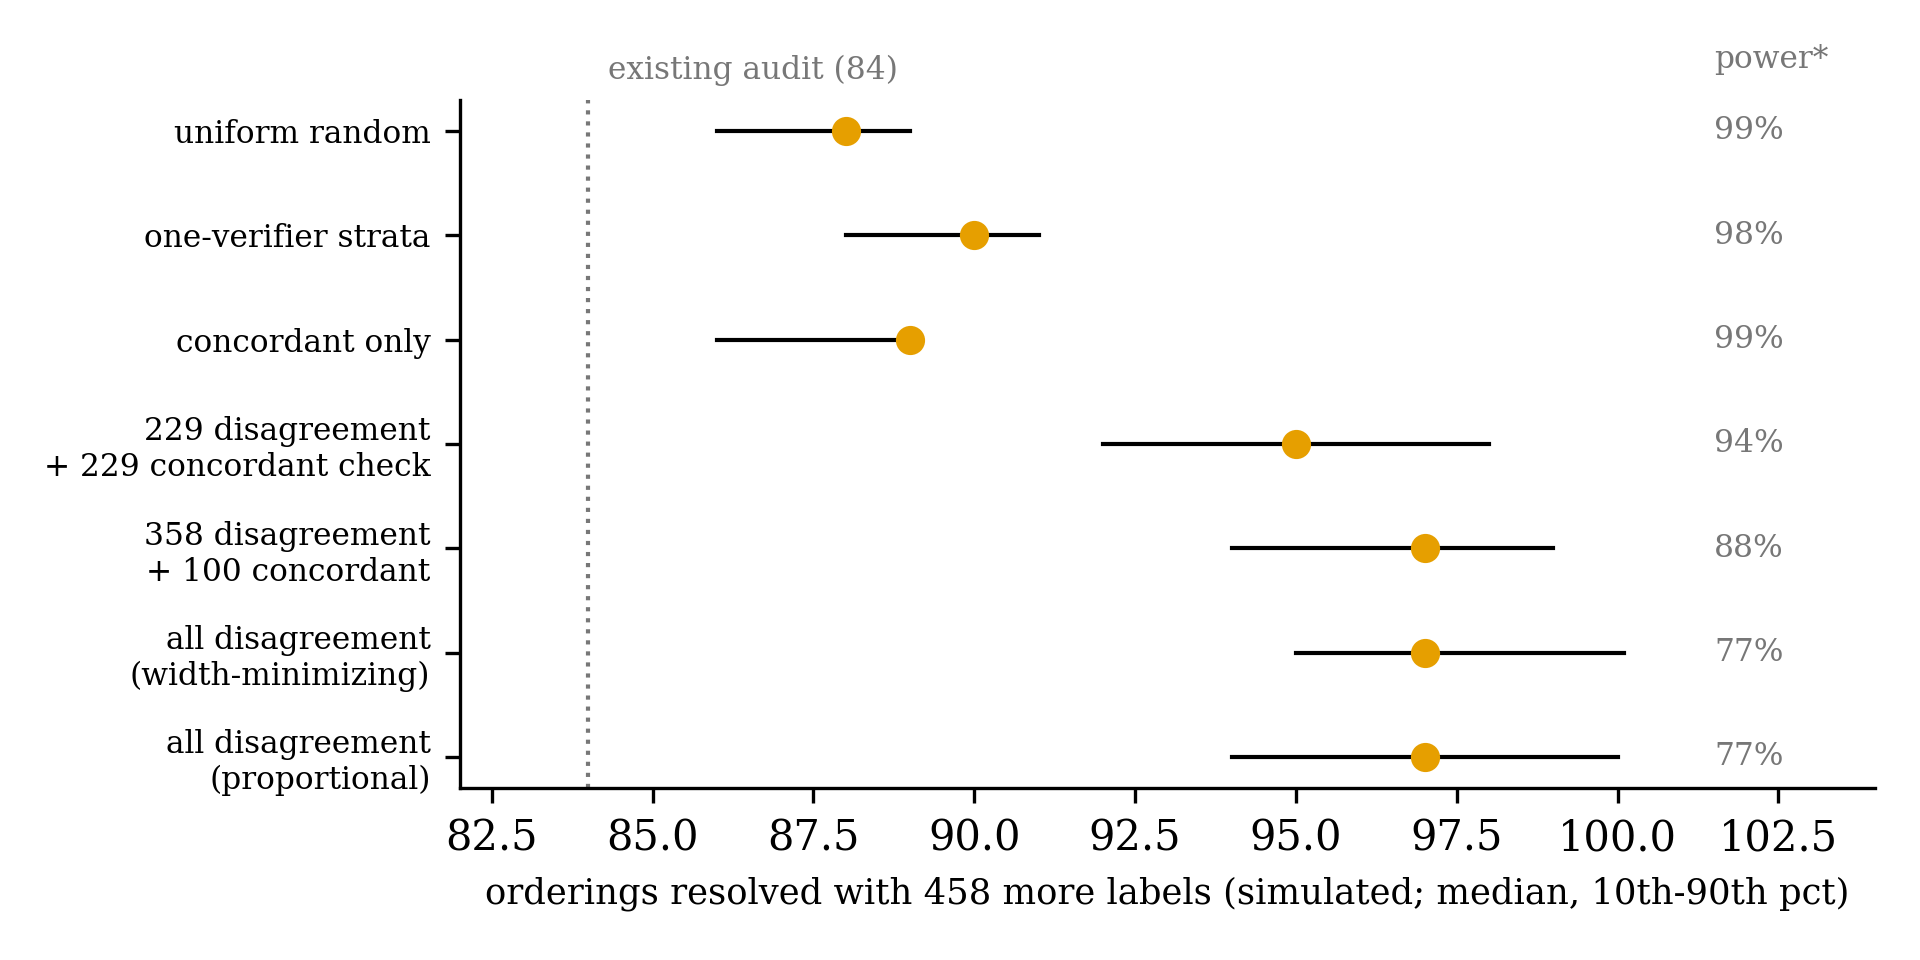
\includegraphics[width=0.80\linewidth]{figD_design_comparison.png}
  \caption{Projected, not observed. Orderings resolved (homogeneous analysis)
  after 458 further labels under each design; \nNRep{} simulated audits per
  design, truths drawn from the existing audit's posterior; median and
  10th--90th percentile. Right column (*): median across models of the
  probability of observing at least one concordant error for a model whose
  concordant error rate is 10\%.}
  \label{fig:designs}
\end{figure}

Figure~\ref{fig:designs} compares designs for 458 further labels under the
same objective. Under homogeneity, spending most labels on disagreements
gives a median of \nDesFullMin--\nDesFullMax{} resolved orderings across
truth scenarios, against \nDesUniform{} for uniform sampling and \nDesOneVer{}
for one-verifier strata; allocations within the disagreement cells differ by
at most a few orderings, so none is uniquely best. The same designs differ
sharply in how well they test the assumption the result rests on: an
all-disagreement design would detect a model with a 10\% concordant error
rate with median probability \nPowFull{} (worst model \nPowFullMin), a
half-and-half design with \nPowBalanced{} (\nPowBalancedMin) while still
reaching \nDesBalancedMin--\nDesBalancedMax. We preregistered the
half-and-half design: 229 disagreement responses stratified by model and 229
concordant responses spread evenly over models. These results are projections
from simulations that draw truths from the same audit used to choose the
design; they are not observed outcomes.

\section{Recommendations}
\label{sec:discussion}

\begin{enumerate}\itemsep2pt
  \item \textbf{Run two verifiers and report their disagreement.} It costs
  nothing, it reverses orderings, and it locates the errors a small audit
  can find.
  \item \textbf{Stratify the audit on joint verifier outcome and state the
  homogeneity assumption.} A ranking claim from a small audit rests on
  treating verifier agreement as equally reliable across models; say so, and
  report how the claim changes as the assumption is relaxed
  (Figure~\ref{fig:assumption}).
  \item \textbf{Spend part of the audit testing that assumption.} Labels on
  concordant responses spread over models are what can falsify it; labels on
  disagreements are what resolve orderings once it holds.
  \item \textbf{Do not pool one verifier's error rates across models to
  support a ranking}, and match the estimator to the sampling: an audit drawn
  within verifier strata estimates $q$ and $r$ (Eq.~\eqref{eq:identity}).
  \item \textbf{Say what the audit measures.} Transcription audits validate
  extraction; semantic equivalence needs a separate check.
\end{enumerate}

\section{Limitations}
\label{sec:limitations}

\begin{enumerate}\itemsep2pt
  \item \textbf{The headline count rests on an untested assumption.}
  \nJointComb{} resolved orderings require concordant error to be homogeneous
  across models; the existing audit supports a low pooled rate but cannot
  test homogeneity, and the count falls quickly as it is relaxed.
  \item \textbf{One benchmark and an older roster.} All results are on
  MATH-Hard with Open LLM Leaderboard v2 models. We did not find a second
  benchmark with two independent live verifiers and an existing human audit;
  the methodology applies wherever two verifiers can be run, but its payoff
  depends on how concentrated verifier error is there.
  \item \textbf{The reference is transcription plus automated comparison},
  with inter-labeler $\kappa$ of 0.61--0.82. The two verifiers share
  normalization code, so their agreement is not independent evidence about
  equivalence errors.
  \item \textbf{The \code{exact\_match}-only cell is barely audited}
  (\nCellZeroOneN{} item) and is bounded by $[0,1]$ per model rather than
  estimated.
  \item \textbf{Design results are projections}, from simulations whose
  truths come from the same audit that motivated the design.
\end{enumerate}

\section{Conclusion}
\label{sec:conclusion}

A small human audit of one verifier, read per model, resolves no MATH-Hard
ordering. Read through the agreement of two verifiers the harness already
runs, it resolves \nJointComb{} of the \nCeiling{} orderings sampling permits,
but only if agreement is equally reliable across models; without that
assumption, resolving as many would take on the order of \nNPLabelsFull{}
labels. The assumption is where a leaderboard's ranking claim now lives, and
the next audit should be designed to test it.


{\small
\bibliographystyle{plainnat}
\bibliography{references}
}

\appendix
\section{Derivations}
\label{sec:appendix-proofs}

\paragraph{Identities.} Conditioning on the verifier outcome,
$P(Y^\ast=1)=P(Y^\ast=1\mid\hat Y=1)P(\hat Y=1)+P(Y^\ast=1\mid\hat Y=0)P(\hat Y=0)
=a(1-q)+(1-a)r$; conditioning on the joint cell gives Eq.~\eqref{eq:joint}.
Bayes' rule gives $\alpha=aq/(1-A^\ast)$ and $\beta=(1-a)r/A^\ast$;
substituting these into $(a-\alpha)/(1-\alpha-\beta)$ recovers $A^\ast$
exactly (checked symbolically in the released code), substituting $q,r$
directly does not.

\paragraph{Sharpness.} $\Delta^\ast=\sum_j k_j\theta_j+\text{const}$ with
coefficients $k_j$ given by census shares ($s_{1c}-s_{2c}$ for a pooled
parameter; $s_{1c}$ and $-s_{2c}$ for model-specific ones). Over a box
$\prod_j[\theta_j^-,\theta_j^+]$ the minimum takes $\theta_j^-$ where
$k_j>0$ and $\theta_j^+$ where $k_j<0$, the maximum the reverse; both are
attained, so the range is sharp.

\paragraph{Pooling one verifier's rates.} With common $(q,r)$,
$\Delta^\ast=(a_1-a_2)(1-q-r)$, whose sign is that of $a_1-a_2$ whenever
$q+r<1$.

\section{Coverage}
\label{sec:appendix-coverage}

Fix an ordering $(1,2)$. Let $E_{\text{aud}}$ be the event that every
estimated parameter it depends on lies in its Clopper--Pearson interval, and
$E_{\text{samp}}$ the event that the benchmark-sampling interval for the
accuracy difference covers its target. The $k$ estimated parameters are
proportions from disjoint audited samples (different cells, or different
models' items), so with per-parameter level $0.975^{1/k}$,
$P(E_{\text{aud}})\ge0.975$ (Clopper--Pearson intervals are conservative, so
the bound holds exactly, not asymptotically). $P(E_{\text{samp}})\approx0.975$
from the normal approximation for a difference of two proportions over
1{,}324 items. On $E_{\text{aud}}$, $\Delta^\ast$ lies in the projected range
(sharpness above); on $E_{\text{aud}}\cap E_{\text{samp}}$, the widened
interval covers the superpopulation difference. By the union bound
$P(E_{\text{aud}}\cap E_{\text{samp}})\ge1-0.025-0.025=0.95$, with no
independence assumption between the audit sample and the benchmark items.
Parameters bounded logically ($[0,1]$ for unaudited disagreement cells, or
the stated bound under bounded heterogeneity) are not estimated and use no
coverage. Under homogeneity the audit part depends only on the two pooled
parameters and so holds for all orderings at once; the simultaneous variant
reported in Section~\ref{sec:results-joint} additionally puts the sampling
part at $0.025/136$ per ordering. The coverage is conditional on the stated
assumption (homogeneity or bounded heterogeneity); it does not account for
the assumption being false.

\section{Why full disagreement auditing stops short of the ceiling}
\label{sec:appendix-census}

If every disagreement response were audited and each model's disagreement
rates equalled the pooled audited value, \nCensusComb{} of the \nCeiling{}
sampling-permitted orderings would be resolved. \nCensusGapShrink{}
sampling-permitted orderings fail, and one ordering that sampling alone does
not resolve becomes resolved. The failures are not for lack of audit
information: correcting the disagreement mass shrinks the accuracy gap below
sampling error, so the pair's \code{score\_boxed} gap is significant but its
corrected gap is not (\nCensusGapShrinkCmdr{} of them involve \code{command-r-v01},
whose \code{score\_boxed} accuracy is mostly disagreement mass). This
projection fixes the disagreement rates at the pooled value and is
illustrative only.

\section{Simulation: plug-in versus two-phase estimator}
\label{sec:appendix-sim}

Finite benchmark of $N=1{,}324$ items; verifier errors drawn with the stated
$(\alpha,\beta)$; audit by simple random sampling within verifier strata
(6--40 items per stratum); 4{,}000 replicates. ``Plug-in'' feeds the audited
stratum rates into $(a-\alpha)/(1-\alpha-\beta)$. Coverage is for the
\v{S}id\'ak-adjusted Wilson projection used in this check.

\begin{center}\small
\resizebox{\linewidth}{!}{\begin{tabular}{@{}lccccc@{}}
\toprule
Scenario ($A^\ast,\alpha,\beta$) & bias, Eq.~(\ref{eq:identity}) & bias, plug-in & cover, Eq.~(\ref{eq:identity}) & cover, plug-in & empty, plug-in \\
\midrule
typical (0.2, 0.01, 0.02) & -0.0001 & -0.027 & 1.000 & 0.998 & 0.00 \\
low accuracy (0.02, 0.01, 0.02) & +0.0002 & -0.560 & 1.000 & 0.237 & 0.60 \\
zero accuracy (0.0, 0.01, 0.0) & +0.0000 & --- & 1.000 & --- & 1.00 \\
high error (0.4, 0.1, 0.15) & -0.0003 & -0.078 & 1.000 & 0.961 & 0.00 \\
perfect verifier (0.2, 0.0, 0.0) & +0.0000 & +0.000 & 1.000 & 1.000 & 0.00 \\
\bottomrule
\end{tabular}
}
\end{center}

\section{One-verifier audit design}
\label{sec:appendix-single}

\begin{figure}[h]
  \centering
  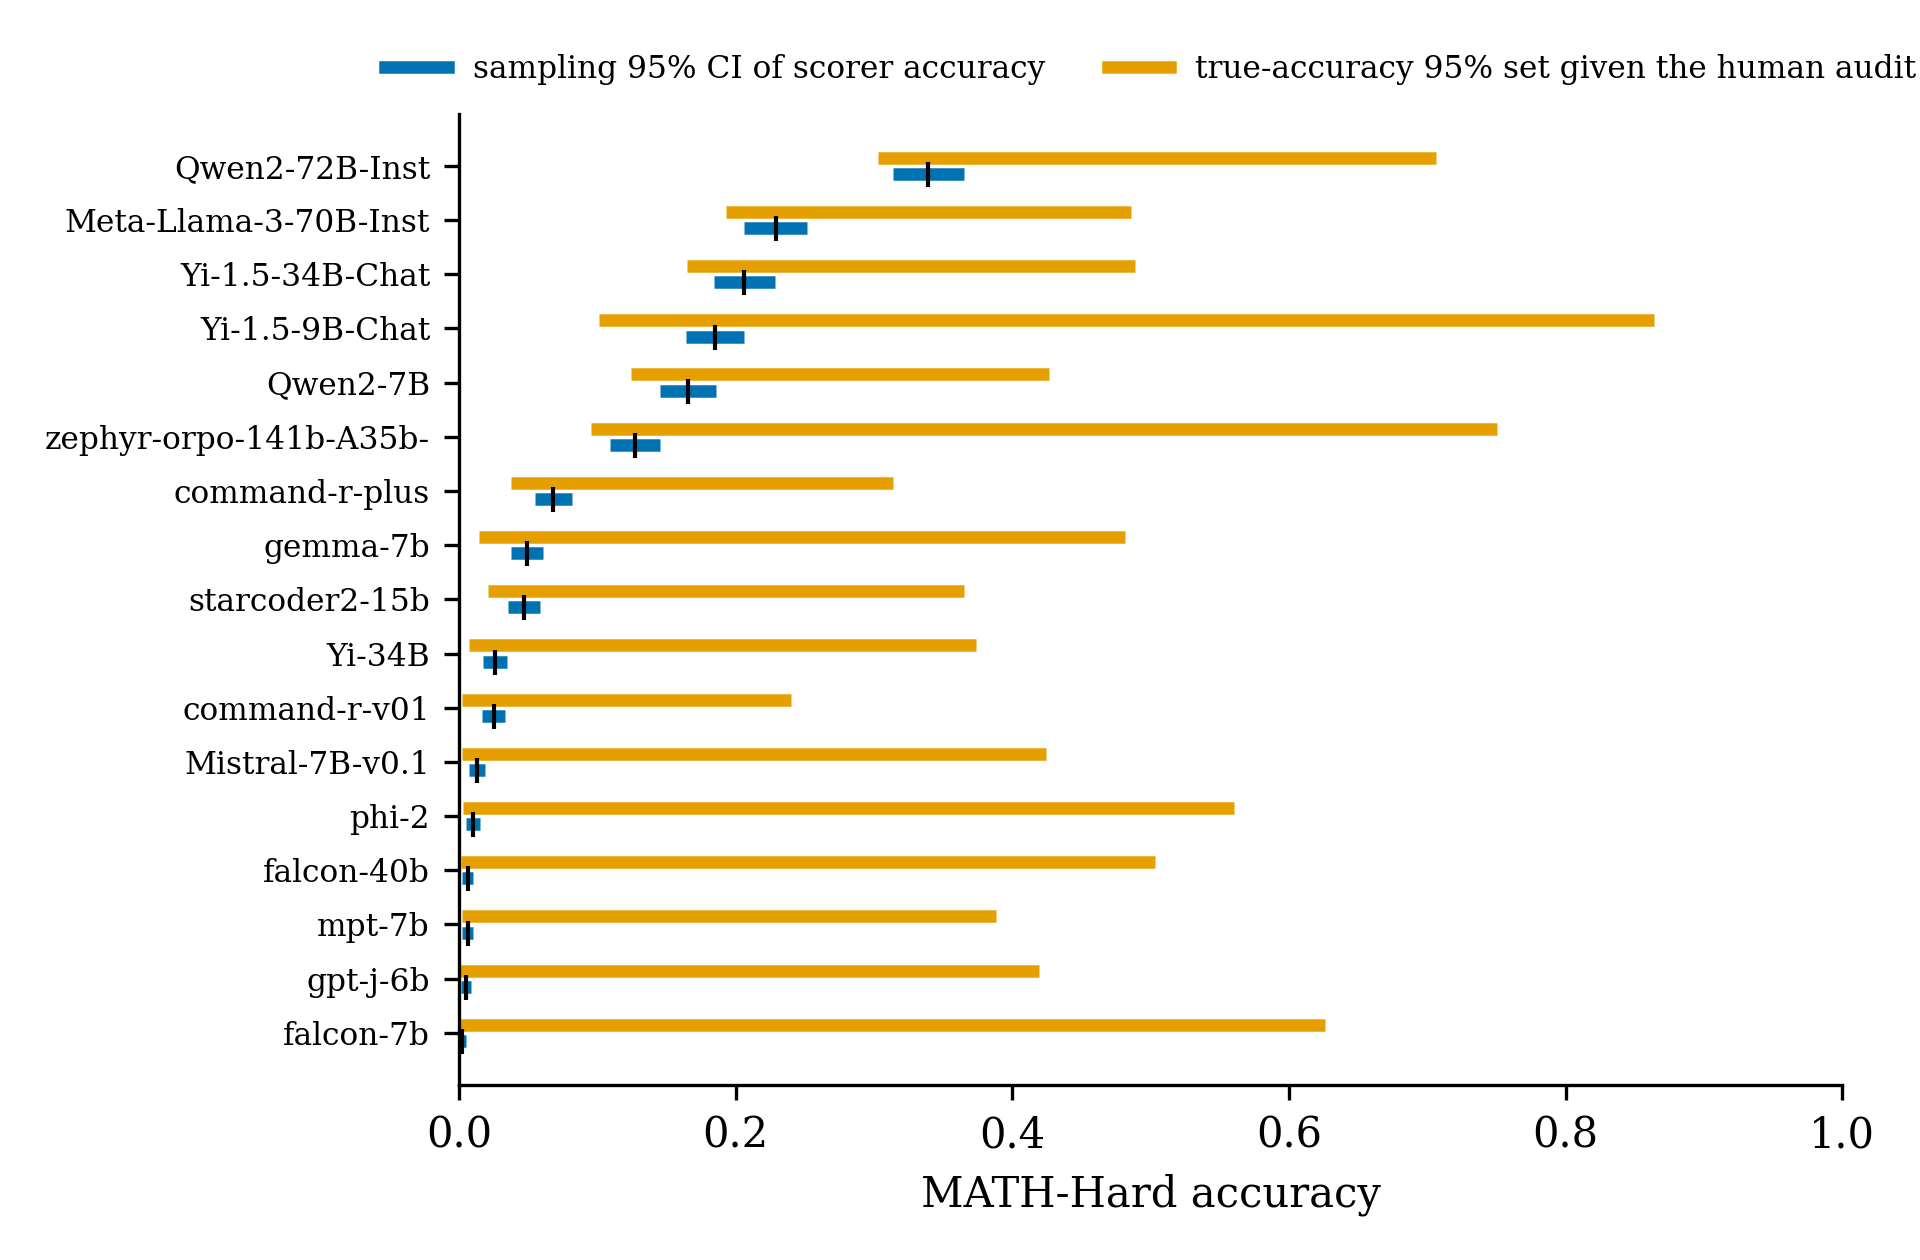
\includegraphics[width=0.50\linewidth]{figA_per_model_intervals.png}
  \caption{Per-model \code{score\_boxed} accuracy: sampling 95\% CI (blue)
  and true-accuracy set from the one-verifier, per-model audit (orange;
  Eq.~\eqref{eq:identity}, \v{S}id\'ak-adjusted Wilson intervals; illustrative).}
  \label{fig:intervals}
\end{figure}

\begin{figure}[h]
  \centering
  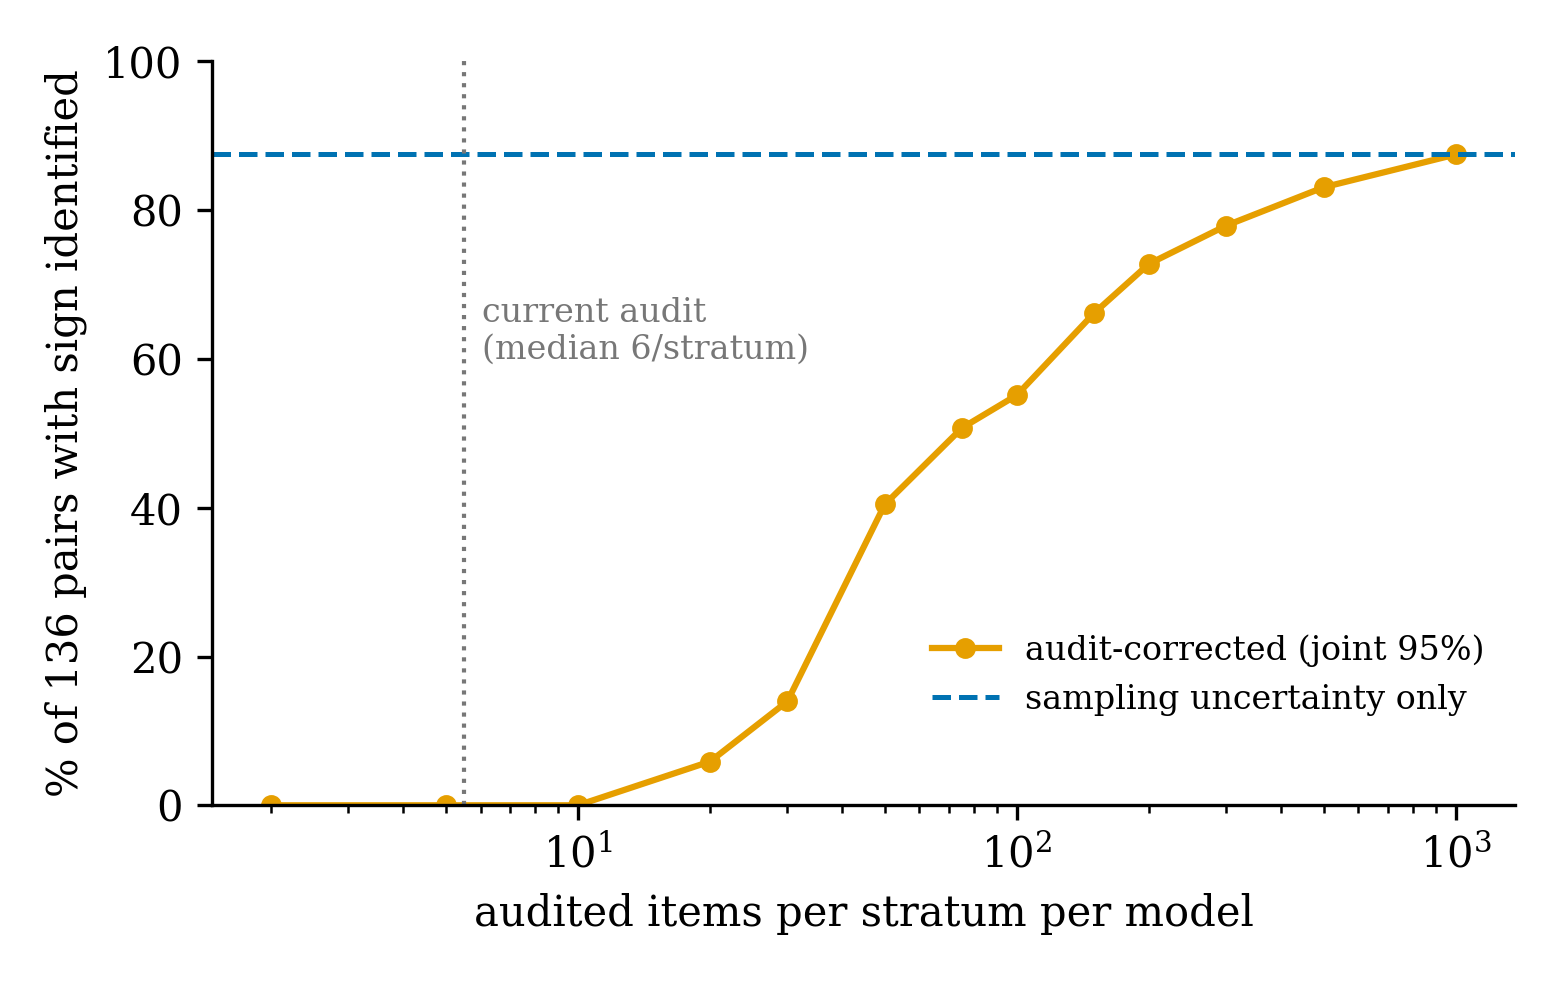
\includegraphics[width=0.44\linewidth]{figB_audit_sizing.png}
  \caption{One verifier, per model (audit only, Wilson): share of orderings
  resolved as audited items per stratum per model grow, each model's
  observed error rates held fixed.}
  \label{fig:sizing}
\end{figure}

For a model with zero observed errors in $n$ items per stratum the Wilson
width is about $z^2/(n+z^2)$; equating it with the sampling width
$2z\sqrt{a(1-a)/N}$ gives $n^\ast\approx(z/2)\sqrt{N/(a(1-a))}-z^2$, i.e.
\nNstarLow, \nNstarMid{} and \nNstarHigh{} items per stratum per model at
$a=0.35,0.20,0.05$. Simulated fresh audits (200 replicates, four truth
scenarios, \nCurTotal{} determinate labels scaled by 1--64) compare five
allocation rules at equal budget; plug-in Neyman resolves nothing at any
budget, and the rule minimizing summed zero-event widths
($n\propto\sqrt{a_m}$, $\sqrt{1-a_m}$) is best or tied. Curves:
\code{reaudit\_results.json}.

\section{Common-mechanism diagnostic}
\label{sec:appendix-mechanism}

\begin{figure}[h]
  \centering
  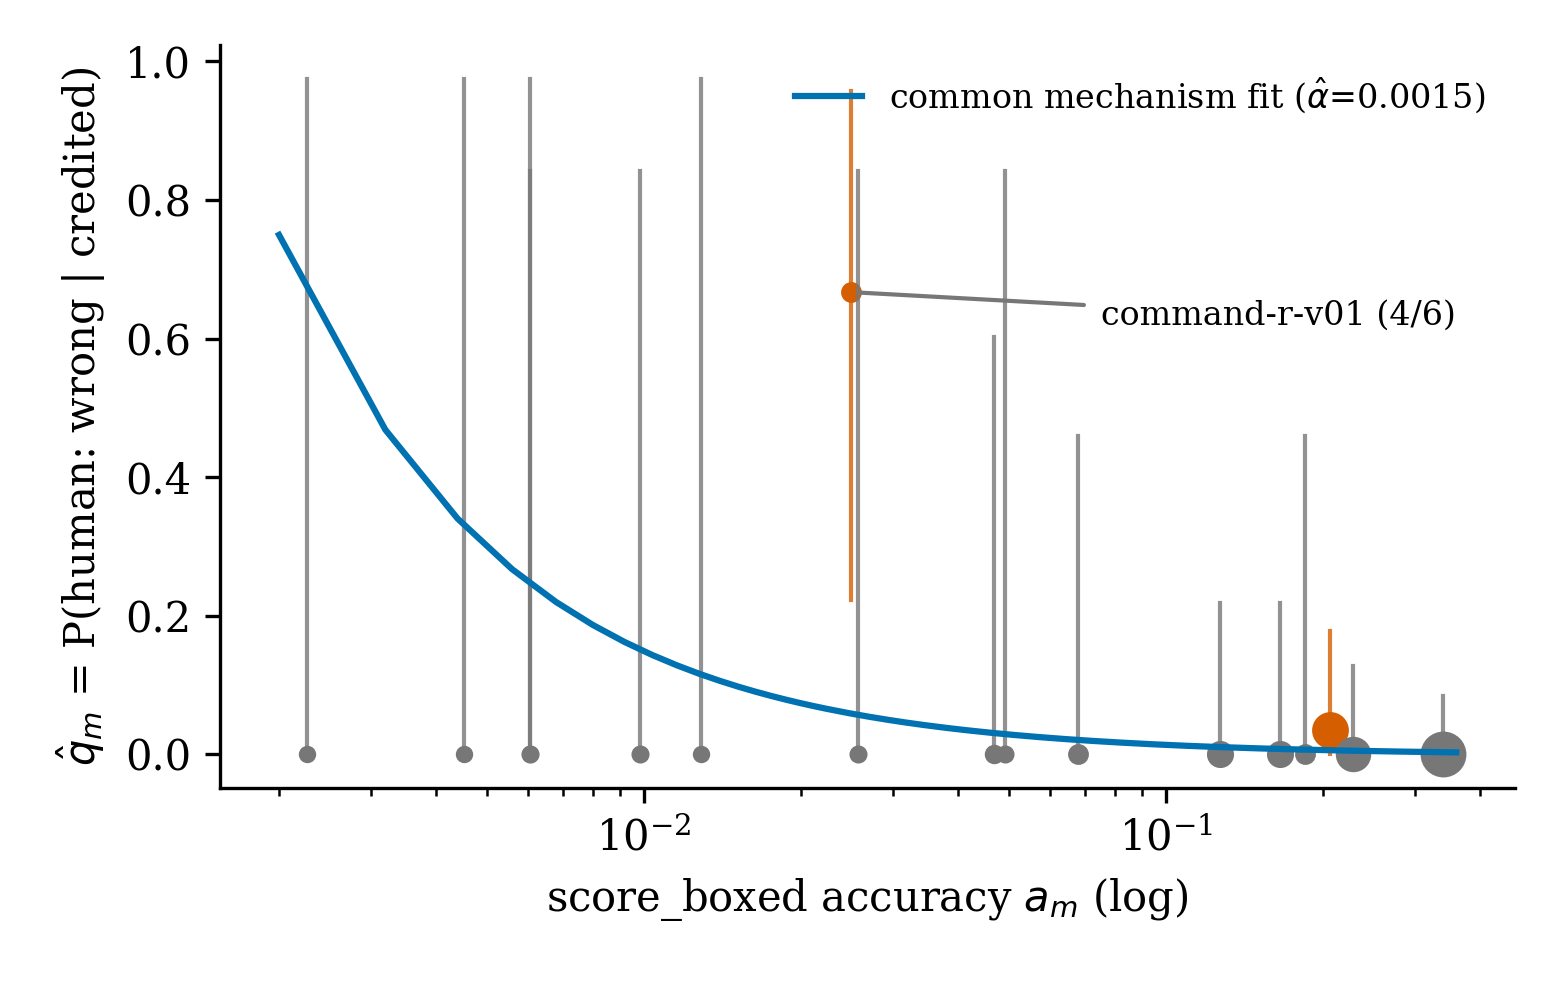
\includegraphics[width=0.44\linewidth]{figC_differential_error.png}
  \caption{Observed $\hat q_m$ (exact 95\% CI) against \code{score\_boxed}
  accuracy, with the rate implied by one common error mechanism.}
  \label{fig:differential}
\end{figure}

Under one $(\alpha,\beta)$ for all models, each model's $(q_m,r_m)$ is
implied by $a_m$. The grid maximum-likelihood fit gives
$\hat\alpha=\nAlphaHat$, $\hat\beta=0$, and a likelihood ratio of \nLR{}
against per-model rates (parametric bootstrap $p=\nLRp$).
\code{command-r-v01} contributes \nCmdrLR{}; leaving it out gives $p=\nLOOCmdrP$,
leaving out any other model gives $p$ between \nLOOOtherPLo{} and
\nLOOOtherPHi{} (500 bootstrap replicates each). The rejection is one model,
whose errors all lie in a disagreement cell; we report it as a diagnostic,
not a general finding.

\section{Per-model audit, one verifier}
\label{sec:appendix-models}

\begin{center}\scriptsize
\resizebox{\linewidth}{!}{\begin{tabular}{@{}lrrrrrc@{}}
\toprule
Model & $a_m$ & false cr./aud. & false rej./aud. & indet. (cr./rej.) & $\hat A^\ast_m$ & 95\% set \\
\midrule
falcon-7b & 0.002 & 0/1 & 0/3 & 1/3 & 0.002 & [0.00, 0.63] \\
gpt-j-6b & 0.005 & 0/1 & 0/7 & 0/1 & 0.005 & [0.00, 0.42] \\
mpt-7b & 0.006 & 0/2 & 0/8 & 0/5 & 0.006 & [0.00, 0.39] \\
falcon-40b & 0.006 & 0/1 & 0/5 & 0/0 & 0.006 & [0.00, 0.50] \\
phi-2 & 0.010 & 0/2 & 0/4 & 0/0 & 0.010 & [0.00, 0.56] \\
Mistral-7B-v0.1 & 0.013 & 0/1 & 0/7 & 0/1 & 0.013 & [0.00, 0.42] \\
c4ai-command-r-v01 & 0.025 & 4/6 & 0/17 & 0/3 & 0.008 & [0.00, 0.24] \\
Yi-34B & 0.026 & 0/2 & 0/9 & 0/0 & 0.026 & [0.01, 0.37] \\
starcoder2-15b & 0.047 & 0/4 & 0/10 & 0/1 & 0.047 & [0.02, 0.36] \\
gemma-7b & 0.049 & 0/2 & 0/6 & 0/1 & 0.049 & [0.01, 0.48] \\
c4ai-command-r-plus & 0.068 & 0/6 & 0/14 & 1/0 & 0.068 & [0.04, 0.31] \\
zephyr-orpo-141b-A35b-v0.1 & 0.127 & 0/15 & 0/2 & 0/0 & 0.127 & [0.10, 0.75] \\
Qwen2-7B & 0.165 & 0/15 & 0/11 & 0/0 & 0.165 & [0.12, 0.43] \\
Yi-1.5-9B-Chat & 0.185 & 0/6 & 0/1 & 8/3 & 0.185 & [0.10, 0.86] \\
Yi-1.5-34B-Chat & 0.206 & 1/29 & 0/9 & 0/1 & 0.199 & [0.16, 0.49] \\
Meta-Llama-3-70B-Instruct & 0.229 & 0/27 & 0/10 & 0/0 & 0.229 & [0.19, 0.49] \\
Qwen2-72B-Instruct & 0.339 & 0/42 & 0/4 & 2/0 & 0.339 & [0.30, 0.71] \\
\bottomrule
\end{tabular}
}
\end{center}

\section{Closest prior work}
\label{sec:appendix-prior}

\begin{center}\footnotesize
\begin{tabular}{@{}p{3.3cm}p{2.3cm}p{2.2cm}ccp{1.9cm}@{}}
\toprule
Work & Estimand & Human sampling & Rank & Two verif. & Allocation \\
\midrule
Two-phase / verification bias \citep{neyman1938contribution,tenenbein1970double,begg1983assessment} & prevalence, Se/Sp & on the cheap result & no & no & phase sizes \\
\citet{lee2026judge} & one model's accuracy & by true label & no & no & between labels \\
Stratified PPI \citep{fisch2024stratified} & a mean metric & stratified & no & no & across strata \\
PP-Ranking \citep{chatzi2024ranking} & rank-sets, many models & random & yes & no & none \\
AutoEval \citep{boyeau2025autoeval} & accuracy, many models & random & partly & no & none \\
This paper & all pairwise orderings & joint-verifier strata & yes & yes & disagreement vs.\ check \\
\bottomrule
\end{tabular}
\end{center}
The estimators here are those of the first row. What differs is the question
(every pairwise ordering of many models), the use of two deterministic
verifiers' agreement as the stratifier, the explicit cross-model homogeneity
assumption and its sensitivity analysis, and an audit design that tests that
assumption.

\section{Reproducibility}
\label{sec:appendix-repro}
\raggedright
Every number in this paper is a macro generated by
\code{scripts/fb\_rebuild\_numbers.py} from result files written by
\code{fb\_joint\_verifier.py}, \code{fb\_reaudit.py},
\code{fb\_rebuild\_analysis.py} and \code{fb\_core\_estimand\_audit.py};
figures by \code{fb\_rebuild\_figures.py}. The estimator is in
\code{flipbudget.pv}, with tests. The preregistered design for the next audit
is \code{TC\_EXPANSION\_PREREGISTRATION.md}, Amendment 3, and its blinded sheet
is \code{labeling/audit\_v2\_l1.csv}.


\end{document}
